\documentclass[main.tex]{subfiles}
\begin{document}

\chapter{Multiple Testing: Family-Wise Error Rate and False Discovery Rate}\label{ch:coklu-test}\chaptermark{Multiple Testing: FWER and FDR}

Neyman--Pearson\index{neyman pearson lemma@Neyman--Pearson lemma} theory (Chapter~\ref{ch:neyman-pearson}) deals with testing a \emph{single} hypothesis and bounds the probability of a type I\index{type i and type ii errors@type I and type II errors} error by $\alpha$. In modern applications, however, hundreds or millions of hypotheses are tested with the same data: differential expression of thousands of genes, dozens of metrics in an A/B experiment, every coefficient in a regression. If each test is performed at level $\alpha=0.05$, then even when all null hypotheses are true, the probability of at least one false rejection in $m=100$ independent tests is $1-0.95^{100}\approx0.994$. In this chapter we study two error criteria. The first is the \emph{family-wise error\index{family wise error rate fwer@family-wise error rate (FWER)} rate} (FWER), which bounds the probability of at least one false rejection; it is controlled by the Bonferroni\index{bonferroni correction@Bonferroni correction} and Holm\index{holm procedure@Holm procedure} procedures. The second is the \emph{false discovery\index{false discovery rate fdr@false discovery rate (FDR)} rate} (FDR), which bounds the expected proportion of false rejections among the rejections; it is controlled by the Benjamini--Hochberg\index{benjamini hochberg procedure@Benjamini--Hochberg procedure} procedure. The central result of the chapter is the short and elegant proof that under independence the BH procedure makes the FDR \emph{exactly} equal to $\pi_0\alpha$.

\section{Definitions}

\begin{definition}[The Multiple Testing Problem]\label{def:coklu-test}
Let null hypotheses $H_1,\dots,H_m$ and their $p$-values $p_1,\dots,p_m$ be given. Let $I_0\subseteq\{1,\dots,m\}$ be the (unknown) set of true null hypotheses, $m_0=|I_0|$ and $\pi_0=m_0/m$. A \emph{multiple testing\index{multiple testing@multiple testing} procedure} produces from the $p$-values a rejection set $\mathcal R\subseteq\{1,\dots,m\}$. $R=|\mathcal R|$ is the total number of rejections and $V=|\mathcal R\cap I_0|$ the number of false rejections (false discoveries).
\begin{center}
\begin{tabular}{lccc}
\toprule
 & Not rejected & Rejected & Total\\
\midrule
True $H_0$ & $m_0-V$ & $V$ & $m_0$\\
False $H_0$ & $m-m_0-(R-V)$ & $R-V$ & $m-m_0$\\
\midrule
Total & $m-R$ & $R$ & $m$\\
\bottomrule
\end{tabular}
\end{center}
\end{definition}

\begin{definition}[Valid $p$-Value]\label{def:gecerli-p}
If for $i\in I_0$, $\P(p_i\le u)\le u$ for every $u\in[0,1]$, then $p_i$ is called a \emph{valid} (super-uniform) $p$-value. The $p$-value of a continuous test statistic under a simple $H_0$ is exactly $\text{Uniform}(0,1)$ (Theorem~\ref{thm:p-uniform}).
\end{definition}

\begin{definition}[Family-Wise Error Rate and False Discovery Rate]\label{def:fwer-fdr}
\[
\mathrm{FWER}=\P(V\ge1),\qquad\mathrm{FDR}=\E\Big[\frac{V}{\max(R,1)}\Big].
\]
The FDR\index{false discovery rate fdr@false discovery rate (FDR)} answers the question ``what proportion of my rejections do I expect to be false?'' \cite{benjamini-hochberg95}. A procedure controls the FWER\index{family wise error rate fwer@family-wise error rate (FWER)} in the \emph{strong sense} if $\mathrm{FWER}\le\alpha$ whatever $I_0$ is, and in the \emph{weak sense} if this holds only when $I_0=\{1,\dots,m\}$.
\end{definition}

\begin{definition}[Three Procedures]\label{def:prosedurler}
Let $p_{(1)}\le\dots\le p_{(m)}$ be the ordered $p$-values and $H_{(k)}$ the corresponding hypotheses.
\begin{itemize}
  \item \emph{Bonferroni\index{bonferroni correction@Bonferroni correction}:} reject every $H_i$ with $p_i\le\alpha/m$.
  \item \emph{Holm\index{holm procedure@Holm procedure}} (step-down) \cite{holm79}: for $k=1,2,\dots$, reject $H_{(k)}$ as long as $p_{(k)}\le\frac{\alpha}{m-k+1}$; stop at the first step where the condition fails.
  \item \emph{Benjamini--Hochberg\index{benjamini hochberg procedure@Benjamini--Hochberg procedure} (BH)} (step-up): $k^*=\max\{k:p_{(k)}\le\alpha k/m\}$ ($k^*=0$ if there is no such $k$); reject $H_{(1)},\dots,H_{(k^*)}$.
\end{itemize}
\end{definition}

\begin{definition}[Adjusted $p$-Values]\label{def:duzeltilmis-p}\index{adjusted p value@adjusted $p$-value|textbf}
The smallest $\alpha$ at which a procedure rejects $H_i$ is called the \emph{adjusted $p$-value} of $H_i$. For the procedures above,
\begin{gather*}
\tilde p_{(k)}^{\text{Bonf}}=\min(1,mp_{(k)}),\qquad
\tilde p_{(k)}^{\text{Holm}}=\min\Big(1,\max_{j\le k}(m-j+1)p_{(j)}\Big),\\
\tilde p_{(k)}^{\text{BH}}=\min\Big(1,\min_{j\ge k}\frac{m\,p_{(j)}}{j}\Big).
\end{gather*}
\end{definition}

\section{Main Theorems and Proofs}

\begin{theorem}[Bonferroni]\label{thm:bonferroni}\index{bonferroni correction@Bonferroni correction}
If the $p$-values are valid, the Bonferroni procedure controls the FWER in the strong sense, whatever the dependence among the $p$-values: $\mathrm{FWER}\le m_0\alpha/m\le\alpha$.
\end{theorem}
\begin{proof}
Boole's inequality\index{boole s inequality@Boole's inequality}: $\P(V\ge1)=\P\Big(\bigcup_{i\in I_0}\{p_i\le\alpha/m\}\Big)\le\sum_{i\in I_0}\P(p_i\le\alpha/m)\le m_0\frac\alpha m$.
\end{proof}

\begin{theorem}[Šidák]\label{thm:sidak}\index{sidák correction@Šidák correction}
If the $p$-values of the true null hypotheses are independent and uniformly distributed, the procedure that performs each test at level $\alpha_m=1-(1-\alpha)^{1/m}$ has FWER $1-(1-\alpha_m)^{m_0}\le\alpha$, with equality when $m_0=m$. Moreover $\alpha_m>\alpha/m$, i.e.\ this procedure is slightly more powerful than Bonferroni \cite{sidak67}.
\end{theorem}
\begin{proof}
By independence, $\P(V=0)=\prod_{i\in I_0}\P(p_i>\alpha_m)=(1-\alpha_m)^{m_0}\ge(1-\alpha_m)^m=1-\alpha$. The inequality $\alpha_m>\alpha/m$ is equivalent to $(1-\alpha/m)^m>1-\alpha$ (Bernoulli's inequality, $m\ge2$, $\alpha\in(0,1)$).
\end{proof}

\begin{theorem}[The Holm Procedure]\label{thm:holm}\index{holm procedure@Holm procedure}
If the $p$-values are valid, the Holm procedure controls the FWER in the strong sense under arbitrary dependence. Moreover, it rejects every hypothesis that Bonferroni rejects.
\end{theorem}
\begin{proof}
Let $m_0\ge1$ (otherwise $V=0$). Define the event $A=\{\min_{i\in I_0}p_i>\alpha/m_0\}$; by Boole's inequality $\P(A^c)\le m_0\cdot\alpha/m_0=\alpha$. We show that on $A$ no true $H_0$ is rejected. Let the first true null hypothesis in the ordered list be in position $j$. Since at most $m-m_0$ hypotheses (all false) precede it, $j\le m-m_0+1$, i.e.\ $m-j+1\ge m_0$. Holm's threshold at step $j$ is $\frac\alpha{m-j+1}\le\frac\alpha{m_0}<p_{(j)}$ (on $A$). Hence the procedure stops at step $j$ at the latest, and no true $H_0$ is rejected: $\P(V\ge1)\le\P(A^c)\le\alpha$.

For the second claim: if Bonferroni rejects $H_{(k)}$, then $p_{(1)}\le\dots\le p_{(k)}\le\alpha/m\le\alpha/(m-j+1)$ for every $j\le k$. So the first $k$ steps of Holm also reject.
\end{proof}

\begin{proposition}[Relation between FDR and FWER]\label{prop:fdr-fwer}\index{false discovery rate fdr@false discovery rate (FDR)}\index{family wise error rate fwer@family-wise error rate (FWER)}
For every procedure, $\mathrm{FDR}\le\mathrm{FWER}$. If all null hypotheses are true ($m_0=m$), $\mathrm{FDR}=\mathrm{FWER}$.
\end{proposition}
\begin{proof}
Since $V\le R$, $\frac{V}{\max(R,1)}\le\I\{V\ge1\}$; take expectations. If $m_0=m$, then $V=R$ and $\frac{V}{\max(R,1)}=\I\{V\ge1\}$.
\end{proof}

Hence FDR control is a weaker guarantee than FWER control; in return it provides much more power. When all nulls are true, the two criteria coincide, and a procedure that controls the FDR controls the FWER in the weak sense.

\begin{lemma}[Structure of BH]\label{lem:bh-yapi}\index{benjamini hochberg procedure@Benjamini--Hochberg procedure}
Fix $i$ and let $R^{(i)}$ denote the number of rejections of the BH procedure when $p_i$ is replaced by $0$ ($R^{(i)}$ depends only on $p_{-i}=(p_j)_{j\ne i}$). Then
\[
H_i\text{ is rejected}\iff p_i\le\frac{\alpha R^{(i)}}m,\qquad\text{and in that case }R=R^{(i)}.
\]
\end{lemma}
\begin{proof}
With $N(t)=\#\{j:p_j\le t\}$ one can write $R=\max\{k:N(\alpha k/m)\ge k\}$ (from the definition of the ordered $p$-values). Decreasing a $p$-value increases $N$ pointwise; hence $R\le R^{(i)}$.

($\Leftarrow$) Let $p_i\le\alpha R^{(i)}/m$. With $p_i=0$ there are at least $R^{(i)}$ $p$-values not exceeding $\alpha R^{(i)}/m$; when $0$ is replaced by $p_i$, the count does not change, since $p_i$ does not exceed this threshold either. So $N(\alpha R^{(i)}/m)\ge R^{(i)}$, hence $R\ge R^{(i)}$ and $R=R^{(i)}$. Since BH rejects every hypothesis whose $p$-value does not exceed $\alpha R/m$, $H_i$ is rejected.

($\Rightarrow$) If $H_i$ is rejected, $p_i\le\alpha R/m\le\alpha R^{(i)}/m$; the first part gives $R=R^{(i)}$.
\end{proof}

\begin{theorem}[Benjamini--Hochberg \cite{benjamini-hochberg95}]\label{thm:bh}\index{benjamini hochberg procedure@Benjamini--Hochberg procedure}
If the $p$-values of the true null hypotheses are $\text{Uniform}(0,1)$ and each is independent of all the other $p$-values, then for the BH procedure
\[
\mathrm{FDR}=\frac{m_0}m\,\alpha=\pi_0\alpha\le\alpha .
\]
If the $p$-values are only valid (super-uniform), $\mathrm{FDR}\le\pi_0\alpha$.
\end{theorem}
\begin{proof}
$\frac{V}{\max(R,1)}=\sum_{i\in I_0}\frac{\I\{H_i\text{ rejected}\}}{\max(R,1)}$. By Lemma~\ref{lem:bh-yapi}, since $R=R^{(i)}\ge1$ when $H_i$ is rejected,
\[
\frac{\I\{H_i\text{ rejected}\}}{\max(R,1)}=\frac{\I\{p_i\le\alpha R^{(i)}/m\}}{R^{(i)}} .
\]
$R^{(i)}$ depends only on $p_{-i}$, and $p_i$ is uniformly distributed independently of $p_{-i}$. Conditioning on $p_{-i}$:
\[
\E\Big[\frac{\I\{p_i\le\alpha R^{(i)}/m\}}{R^{(i)}}\,\Big|\,p_{-i}\Big]=\frac{\P(p_i\le\alpha R^{(i)}/m\mid p_{-i})}{R^{(i)}}=\frac{\alpha R^{(i)}/m}{R^{(i)}}=\frac\alpha m .
\]
($R^{(i)}\ge1$ always, because with $p_i=0$ at least $H_i$ is rejected.) Taking expectations and summing over $i\in I_0$ gives $\mathrm{FDR}=m_0\alpha/m$. For super-uniform $p$-values the middle equality becomes $\le$.
\end{proof}

\begin{theorem}[Arbitrary Dependence: Benjamini--Yekutieli \cite{benjamini-yekutieli01}]\label{thm:by}\index{benjamini yekutieli procedure@Benjamini--Yekutieli procedure}
If the $p$-values are valid and the dependence is arbitrary, then applying the BH procedure with $\alpha/c_m$ instead of $\alpha$ gives $\mathrm{FDR}\le\pi_0\alpha$, where $c_m=\sum_{k=1}^m\frac1k\approx\ln m+0.577$. Moreover, if the test statistics have positive regression dependence (PRDS), for example one-sided tests with positively correlated multivariate normal\index{multivariate normal distribution@multivariate normal distribution} statistics, uncorrected BH already gives $\mathrm{FDR}\le\pi_0\alpha$.
\end{theorem}

\section{Worked Examples}

\begin{example}[Ten $p$-Values]\label{ex:on-p}
$\alpha=0.05$ and the ordered $p$-values: $0.001$; $0.008$; $0.039$; $0.041$; $0.042$; $0.060$; $0.074$; $0.205$; $0.212$; $0.216$.
\begin{itemize}
  \item Uncorrected: the first five hypotheses, with $p\le0.05$, are rejected.
  \item Bonferroni\index{bonferroni correction@Bonferroni correction}: the threshold is $0.005$; only $H_{(1)}$.
  \item Holm\index{holm procedure@Holm procedure}: $0.001\le0.05/10$, so $H_{(1)}$ is rejected; since $0.008>0.05/9=0.0056$, we stop. Again only $H_{(1)}$.
  \item BH\index{benjamini hochberg procedure@Benjamini--Hochberg procedure}: the thresholds are $0.005k$. $p_{(2)}=0.008\le0.010$, but for $k\ge3$, $p_{(k)}>0.005k$ ($0.039>0.015$, $0.041>0.020$, \ldots, $0.216>0.050$). $k^*=2$; $H_{(1)}$ and $H_{(2)}$ are rejected.
\end{itemize}
Although the three $p$-values around $0.04$ look ``significant'' on their own, none of them is rejected after the multiple testing\index{multiple testing@multiple testing} correction.
\end{example}

\begin{example}[When to Use Which?]\label{ex:hangisi}
For a small number of hypotheses where every false discovery\index{false discovery rate fdr@false discovery rate (FDR)} has serious consequences, such as the primary and secondary endpoints of a drug trial, FWER\index{family wise error rate fwer@family-wise error rate (FWER)} control is appropriate. Holm is always better than Bonferroni (Theorem~\ref{thm:holm}) and works under the same assumption. In exploratory screening (genomics, imaging), by contrast, the rejections form a list of \emph{candidates} to be validated in later experiments; here it is enough that most of the list is correct, and FDR control is appropriate. For $m=1000$ the Bonferroni threshold is $5\times10^{-5}$, i.e.\ $z\approx3.89$. Most real effects of size $3\sigma$ cannot pass this threshold.
\end{example}

\section{Computational Applications}

\subsection{FWER, FDR and Power}
Out of $m=1000$ one-sided $z$-tests, $m_1=100$ have a real effect $\mu=3$; the tests are independent. We compare four procedures with $M=2000$ replications.

\pycode{code/ch22/c22_1_bonferroni_holm_bh.py}
\begin{lstlisting}[style=output]
m = 1000, number of false H0 m1 = 100, effect = 3.0, alpha = 0.05, replications = 2000
Method       |  FWER  |  FDR   | power  | mean rej.
Uncorrected  | 1.000  | 0.3296 | 0.912  |   136.3
Bonferroni   | 0.046  | 0.0024 | 0.185  |    18.6
Holm         | 0.046  | 0.0024 | 0.187  |    18.7
BH           | 0.943  | 0.0456 | 0.607  |    63.7
theoretical FDR for BH = pi0 * alpha = 0.0450
\end{lstlisting}

For the uncorrected test the FWER\index{family wise error rate fwer@family-wise error rate (FWER)} is $1$, and about a third of the rejections are false discoveries. Bonferroni\index{bonferroni correction@Bonferroni correction} and Holm\index{holm procedure@Holm procedure} keep the FWER below $0.05$ but find only $19\%$ of the real effects. Since $m_0=900$ is large, Holm's advantage over Bonferroni is negligible here. The FDR\index{false discovery rate fdr@false discovery rate (FDR)} of BH\index{benjamini hochberg procedure@Benjamini--Hochberg procedure} agrees within Monte Carlo error with the theoretical value $\pi_0\alpha=0.045$ (Theorem~\ref{thm:bh}), and its power is more than three times larger. The price is that it makes at least one false discovery in almost every replication ($\mathrm{FWER}\approx0.94$): BH does not guarantee ``make no errors'' but ``keep the proportion of errors small''.

\subsection{Dependence and a Visual Interpretation of BH}
Suppose all null hypotheses are true and the test statistics are equicorrelated ($\rho$) normal; two-sided $p$-values are used.

\pycode{code/ch22/c22_2_dependence_and_bh.py}
\begin{lstlisting}[style=output]
All H0 true (m = 100); equicorrelated normal test statistics
 rho | Bonferroni FWER | uncorrected FWER | BH FDR (= FWER)
 0.0 |      0.0515     |      0.9932      |     0.0532
 0.3 |      0.0420     |      0.9390      |     0.0457
 0.6 |      0.0220     |      0.6412      |     0.0278
 0.9 |      0.0065     |      0.2195      |     0.0195
Example data: BH rejected 11 hypotheses; real effects: 11, false discoveries: 0. Bonferroni rejections: 8.
\end{lstlisting}

\begin{figure}[h]
\centering
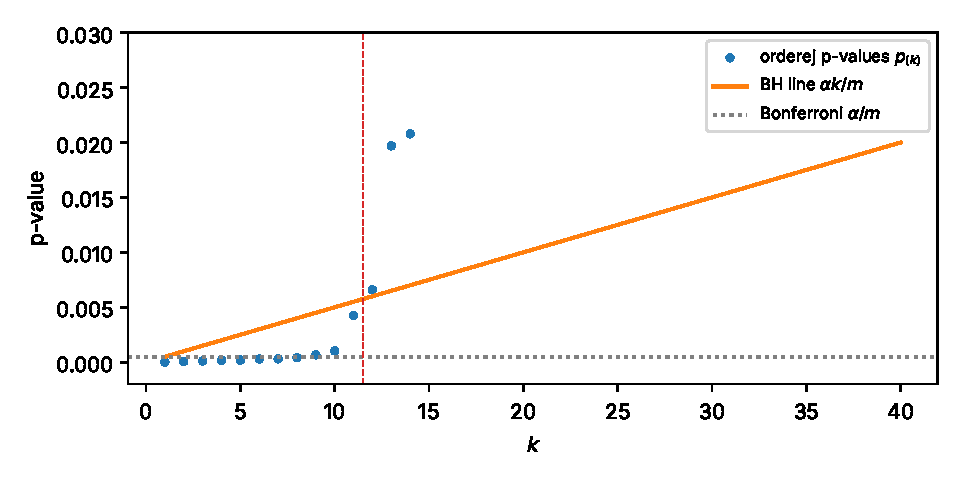
\includegraphics[width=0.8\textwidth]{figures/bh_dogrusu.pdf}
\caption{The BH procedure: find the \emph{last} $k$ at which the ordered $p$-values lie below the line $\alpha k/m$, and reject all hypotheses up to it (dashed vertical line). The Bonferroni threshold is the horizontal dotted line.}
\end{figure}

As the dependence increases, Bonferroni and BH become conservative: at $\rho=0.9$ the tests carry almost the same information, the ``effective number of tests'' is much smaller than $m$, and Boole's inequality\index{boole s inequality@Boole's inequality} becomes crude. The FWER of the uncorrected test falls for the same reason. Since all nulls are true, the FDR of BH equals its FWER (Proposition~\ref{prop:fdr-fwer}), and under independence it is very close to $\alpha$. In this simulation the FDR of BH stayed below $\alpha$ with two-sided $p$-values as well. For one-sided tests the same correlation structure satisfies the PRDS condition, and the guarantee is exact by Theorem~\ref{thm:by}.

\section{Comments and Notes}

\begin{remark}[Estimating $\pi_0$]
Theorem~\ref{thm:bh} shows that BH\index{benjamini hochberg procedure@Benjamini--Hochberg procedure} in fact controls at level $\pi_0\alpha$; if $\pi_0$ is small the procedure is more conservative than necessary. \emph{Adaptive} procedures first estimate $\pi_0$; for example, based on the observation that large $p$-values come almost entirely from true nulls, $\hat\pi_0=\#\{p_i>\lambda\}/(m(1-\lambda))$ is used. They then apply BH with $\alpha/\hat\pi_0$.
\end{remark}

\begin{remark}[Bayesian Interpretation]
In the two-group mixture model ($p_i$ comes from $\text{Uniform}(0,1)$ with probability $\pi_0$ and from an alternative distribution $F_1$ with probability $1-\pi_0$), $\P(H_i\text{ true}\mid p_i\le t)=\pi_0t/F(t)$, where $F=\pi_0t+(1-\pi_0)F_1$. BH can be interpreted as estimating $F(t)$ by the empirical CDF\index{empirical distribution function@empirical distribution function} and choosing the largest threshold that keeps this \emph{tail-area false discovery\index{false discovery rate fdr@false discovery rate (FDR)} rate} below $\alpha$. This is the application of the posterior-probability reasoning of Chapter~\ref{ch:bayes} to many parallel problems (empirical Bayes\index{empirical bayes@empirical Bayes}).
\end{remark}

\begin{remark}[Selective Inference]
A more insidious form of the multiple testing\index{multiple testing@multiple testing} problem is choosing which hypothesis to test after looking at the data: reporting the subgroup that shows the largest effect, or giving ordinary confidence intervals for coefficients selected after model selection\index{model selection@model selection}. After selection, ordinary $p$-values and intervals are not valid. Simple safe solutions are data splitting and pre-registration. Theoretical solutions perform inference conditional on the selection event.
\end{remark}

% --- CHAPTER SUMMARY ---
\section{Chapter Summary}
\begin{summary}
\begin{itemize}
  \item When many tests are performed simultaneously, an error measure must be chosen: the family-wise error rate (FWER) or the false discovery rate (FDR) (Definition~\ref{def:fwer-fdr}). Always $\mathrm{FDR}\le\mathrm{FWER}$; if all null hypotheses are true, the two are equal (Proposition~\ref{prop:fdr-fwer}).
  \item The Bonferroni correction controls the FWER under every dependence structure (Theorem~\ref{thm:bonferroni}). The Šidák correction is slightly more powerful under independence (Theorem~\ref{thm:sidak}). The Holm procedure (Theorem~\ref{thm:holm}) uniformly dominates Bonferroni.
  \item The Benjamini--Hochberg procedure keeps the FDR at level $\pi_0\alpha$ for independent $p$-values (Theorem~\ref{thm:bh}). Under arbitrary dependence it is applied with $\alpha/c_m$ (Theorem~\ref{thm:by}), where $c_m\approx\ln m$.
  \item Adjusted $p$-values (Definition~\ref{def:duzeltilmis-p}) make it possible to report the result for each hypothesis rather than for a single threshold.
  \item With thousands of tests, FWER control reduces power drastically. FDR control, by accepting a small number of false discoveries, finds a much larger fraction of the real effects.
\end{itemize}
\end{summary}
% --- END OF CHAPTER SUMMARY ---

\paragraph{Further reading.} \cite{benjamini-hochberg95,holm79,benjamini-yekutieli01}; at textbook level, \cite[Chapter~9]{lehmann-romano} and \cite[Section~10.7]{wasserman}.

\section{Exercises}

\begin{exercise}\label{exr:22-1}
For the $p$-values of Example~\ref{ex:on-p}, compute the Bonferroni, Holm and BH adjusted $p$-values (Definition~\ref{def:duzeltilmis-p}). Verify that the hypotheses each procedure rejects at $\alpha=0.05$ are those with adjusted $p$-value $\le0.05$. How many hypotheses does BH reject with $\alpha=0.10$?
\hfill\hyperref[coz:22-1]{\footnotesize$\rightarrow$\,Solution}
\end{exercise}

\begin{exercise}\label{exr:22-2}
Show that for $m$ independent null hypotheses, all true, the FWER of the uncorrected test is $1-(1-\alpha)^m$. Compute its values for $\alpha=0.05$ and $m=1,5,20,100$. Show that $m\alpha_m\to-\ln(1-\alpha)$ as $m\to\infty$ ($\alpha_m$: the Šidák level), and compare this with Bonferroni.
\hfill\hyperref[coz:22-2]{\footnotesize$\rightarrow$\,Solution}
\end{exercise}

\begin{exercise}\label{exr:22-3}
Give an example of a procedure that controls the FWER in the weak sense but not in the strong sense. (Hint: consider the procedure that first tests ``is there at least one effect?'' with Bonferroni and, in case of rejection, rejects all hypotheses with $p_i\le\alpha$.)
\hfill\hyperref[coz:22-3]{\footnotesize$\rightarrow$\,Solution}
\end{exercise}

\begin{exercise}\label{exr:22-4}
Let there be $m=2$ independent tests with $m_0=1$. If the $p$-value of the false hypothesis is $0$ with probability $1$ (a very powerful test), verify by direct computation that the FDR of the BH procedure is $\alpha/2$.
\hfill\hyperref[coz:22-4]{\footnotesize$\rightarrow$\,Solution}
\end{exercise}

\chapterlinks{22}

\end{document}
